% =============================================================
% Annexure J: Multi-Seed Robustness Supplementary Figures
% =============================================================
\section{Multi-Seed Robustness Supplementary Figures}
\label{annexure:multiseed}

This annexure presents supplementary diagnostic figures for the
multi-seed robustness analyses discussed in
Chapter~\ref{sec:results}.  The figures below provide detailed
visual evidence supporting the cross-seed stability claims
summarised in the main text.

% -------------------------------------------------------------
\subsection{DNN Training Convergence Across Seeds}
\label{annexure:multiseed_training}

Figures~\ref{fig:dnn_multiseed_train_loss_annex}
to~\ref{fig:dnn_multiseed_epoch_vs_r2_annex} display the training
convergence behaviour of the FunnelDNN across five random seeds
(seeds 42, 123, 456, 789 and 1024).

\begin{figure}[H]
\centering
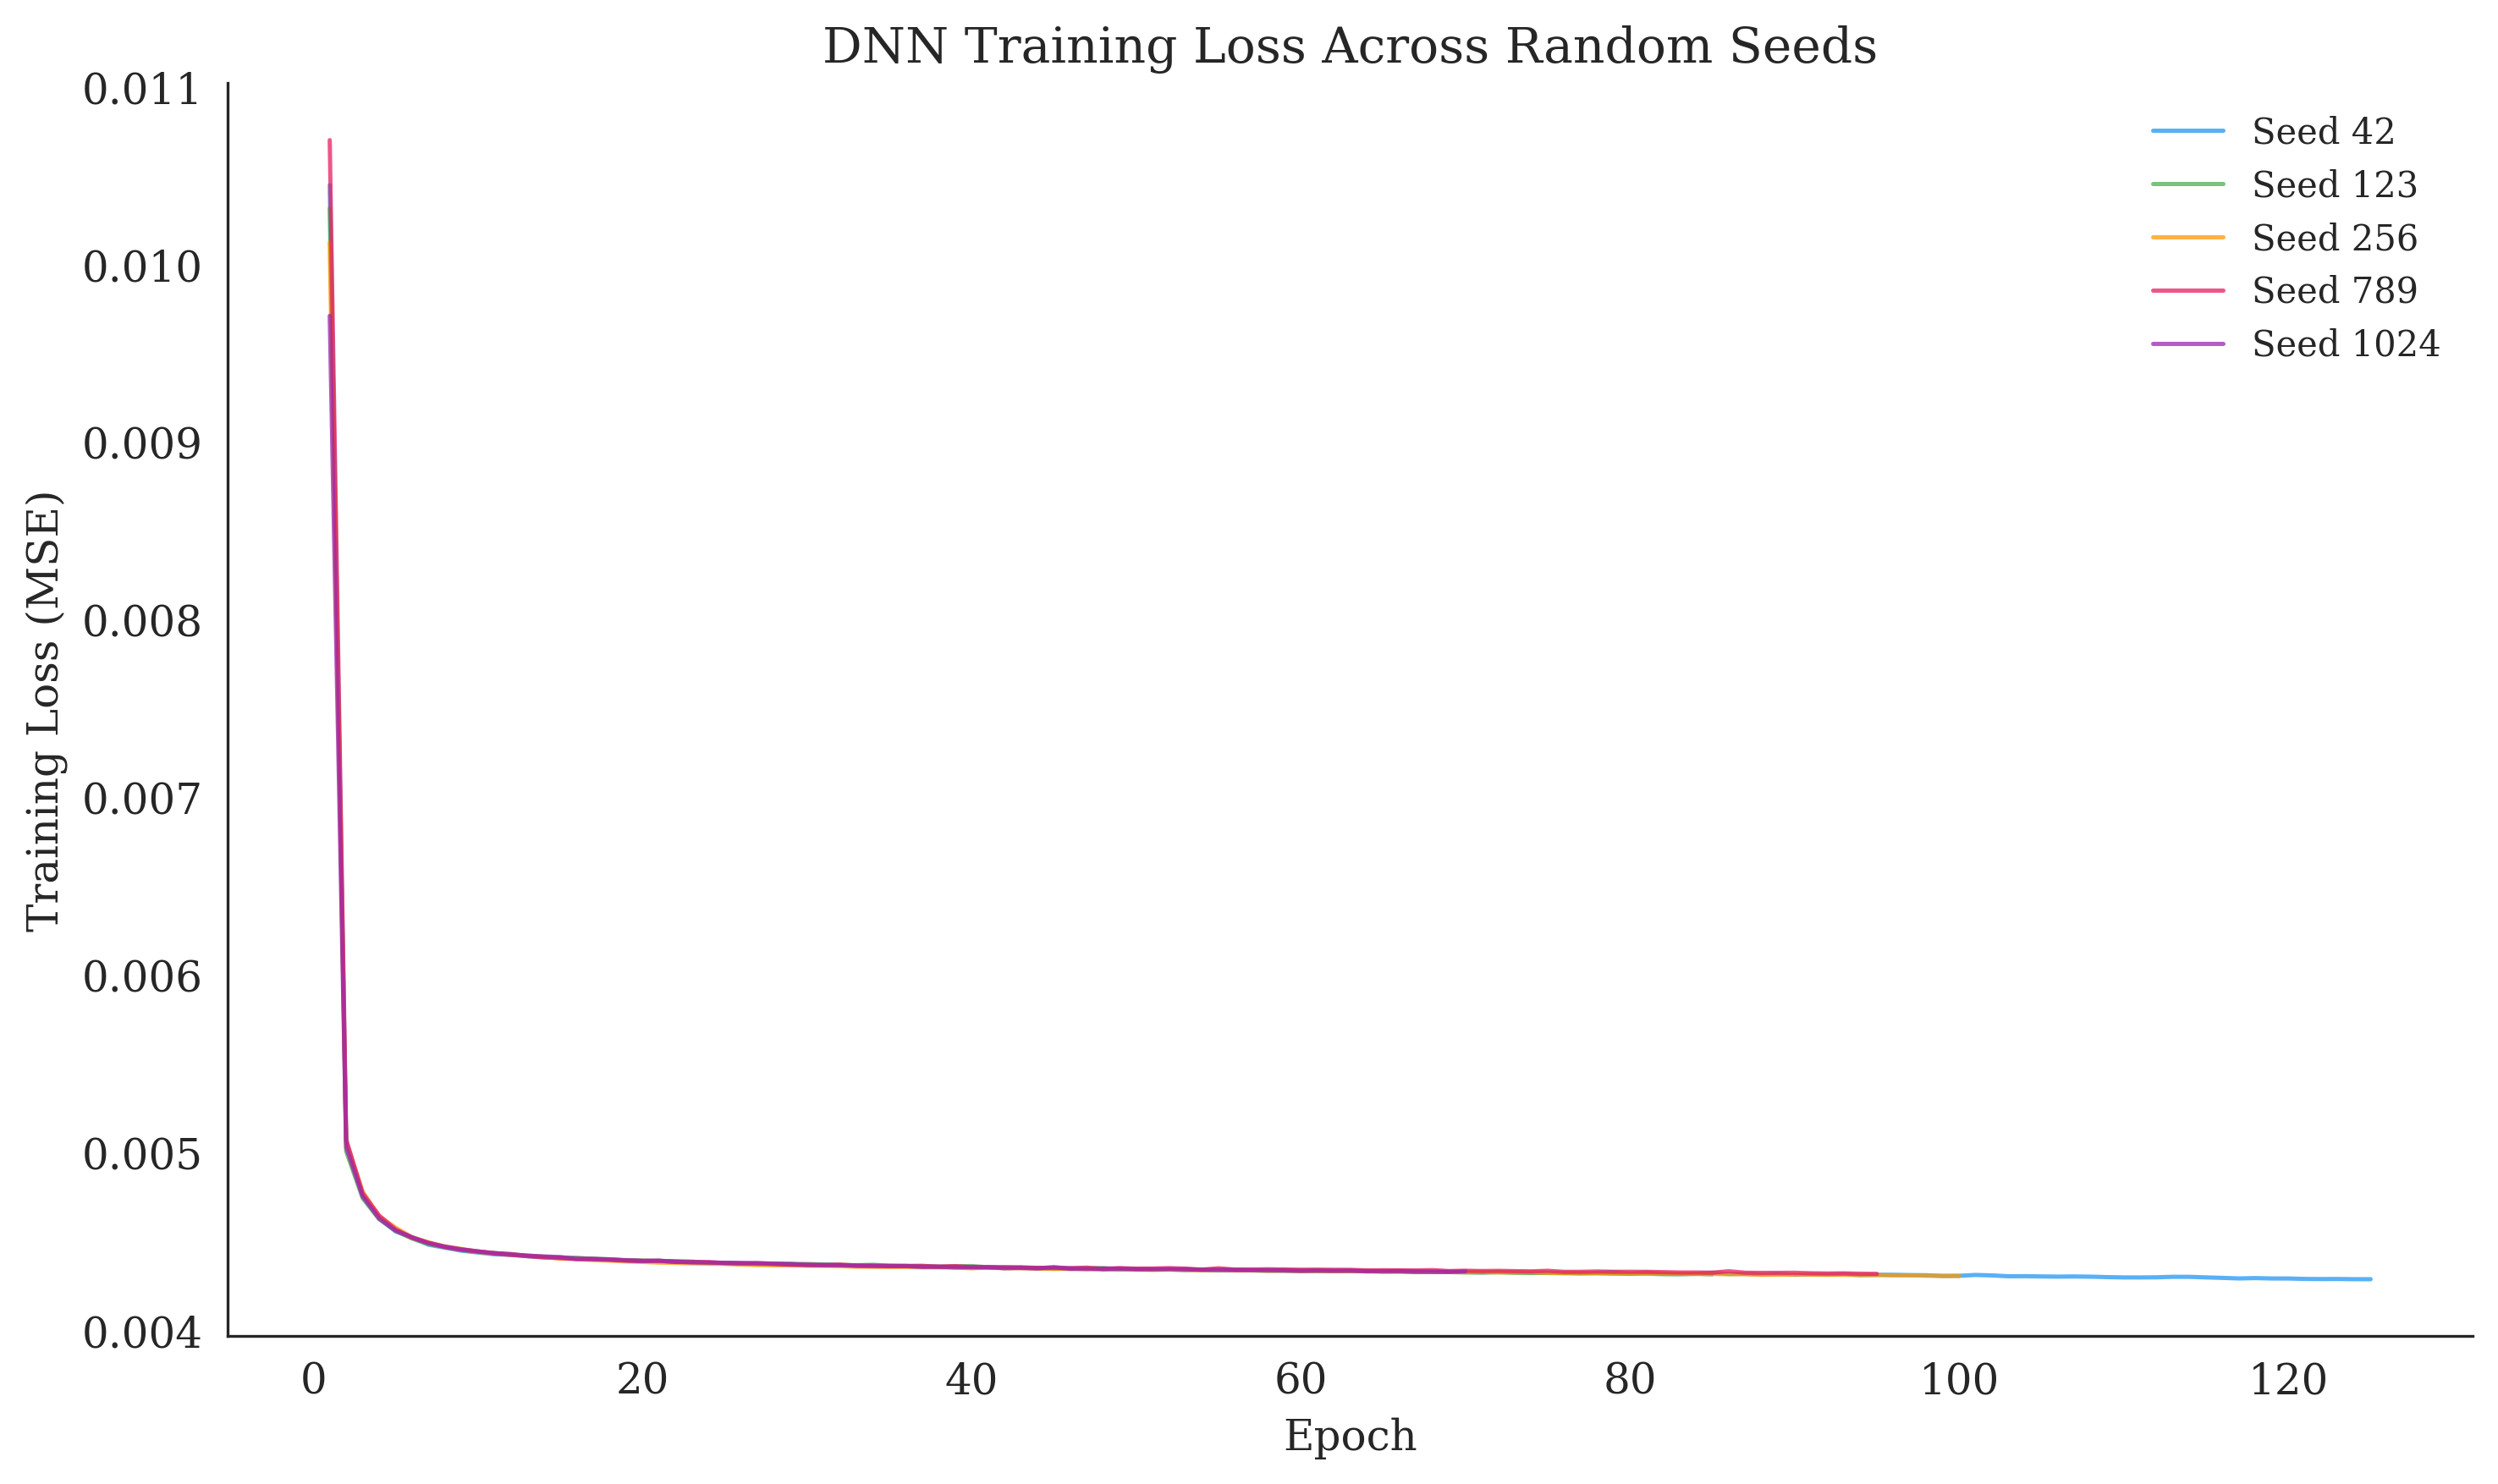
\includegraphics[width=0.92\textwidth]{Thesis/Chapter 4/Figures/fig_dnn_multiseed_train_loss.png}
\caption{Training loss trajectories across five random seeds.  All
five seeds converge to the same loss plateau, confirming that the
optimisation landscape does not trap any seed in a materially
different local minimum.}
\label{fig:dnn_multiseed_train_loss_annex}
\end{figure}

\begin{figure}[H]
\centering
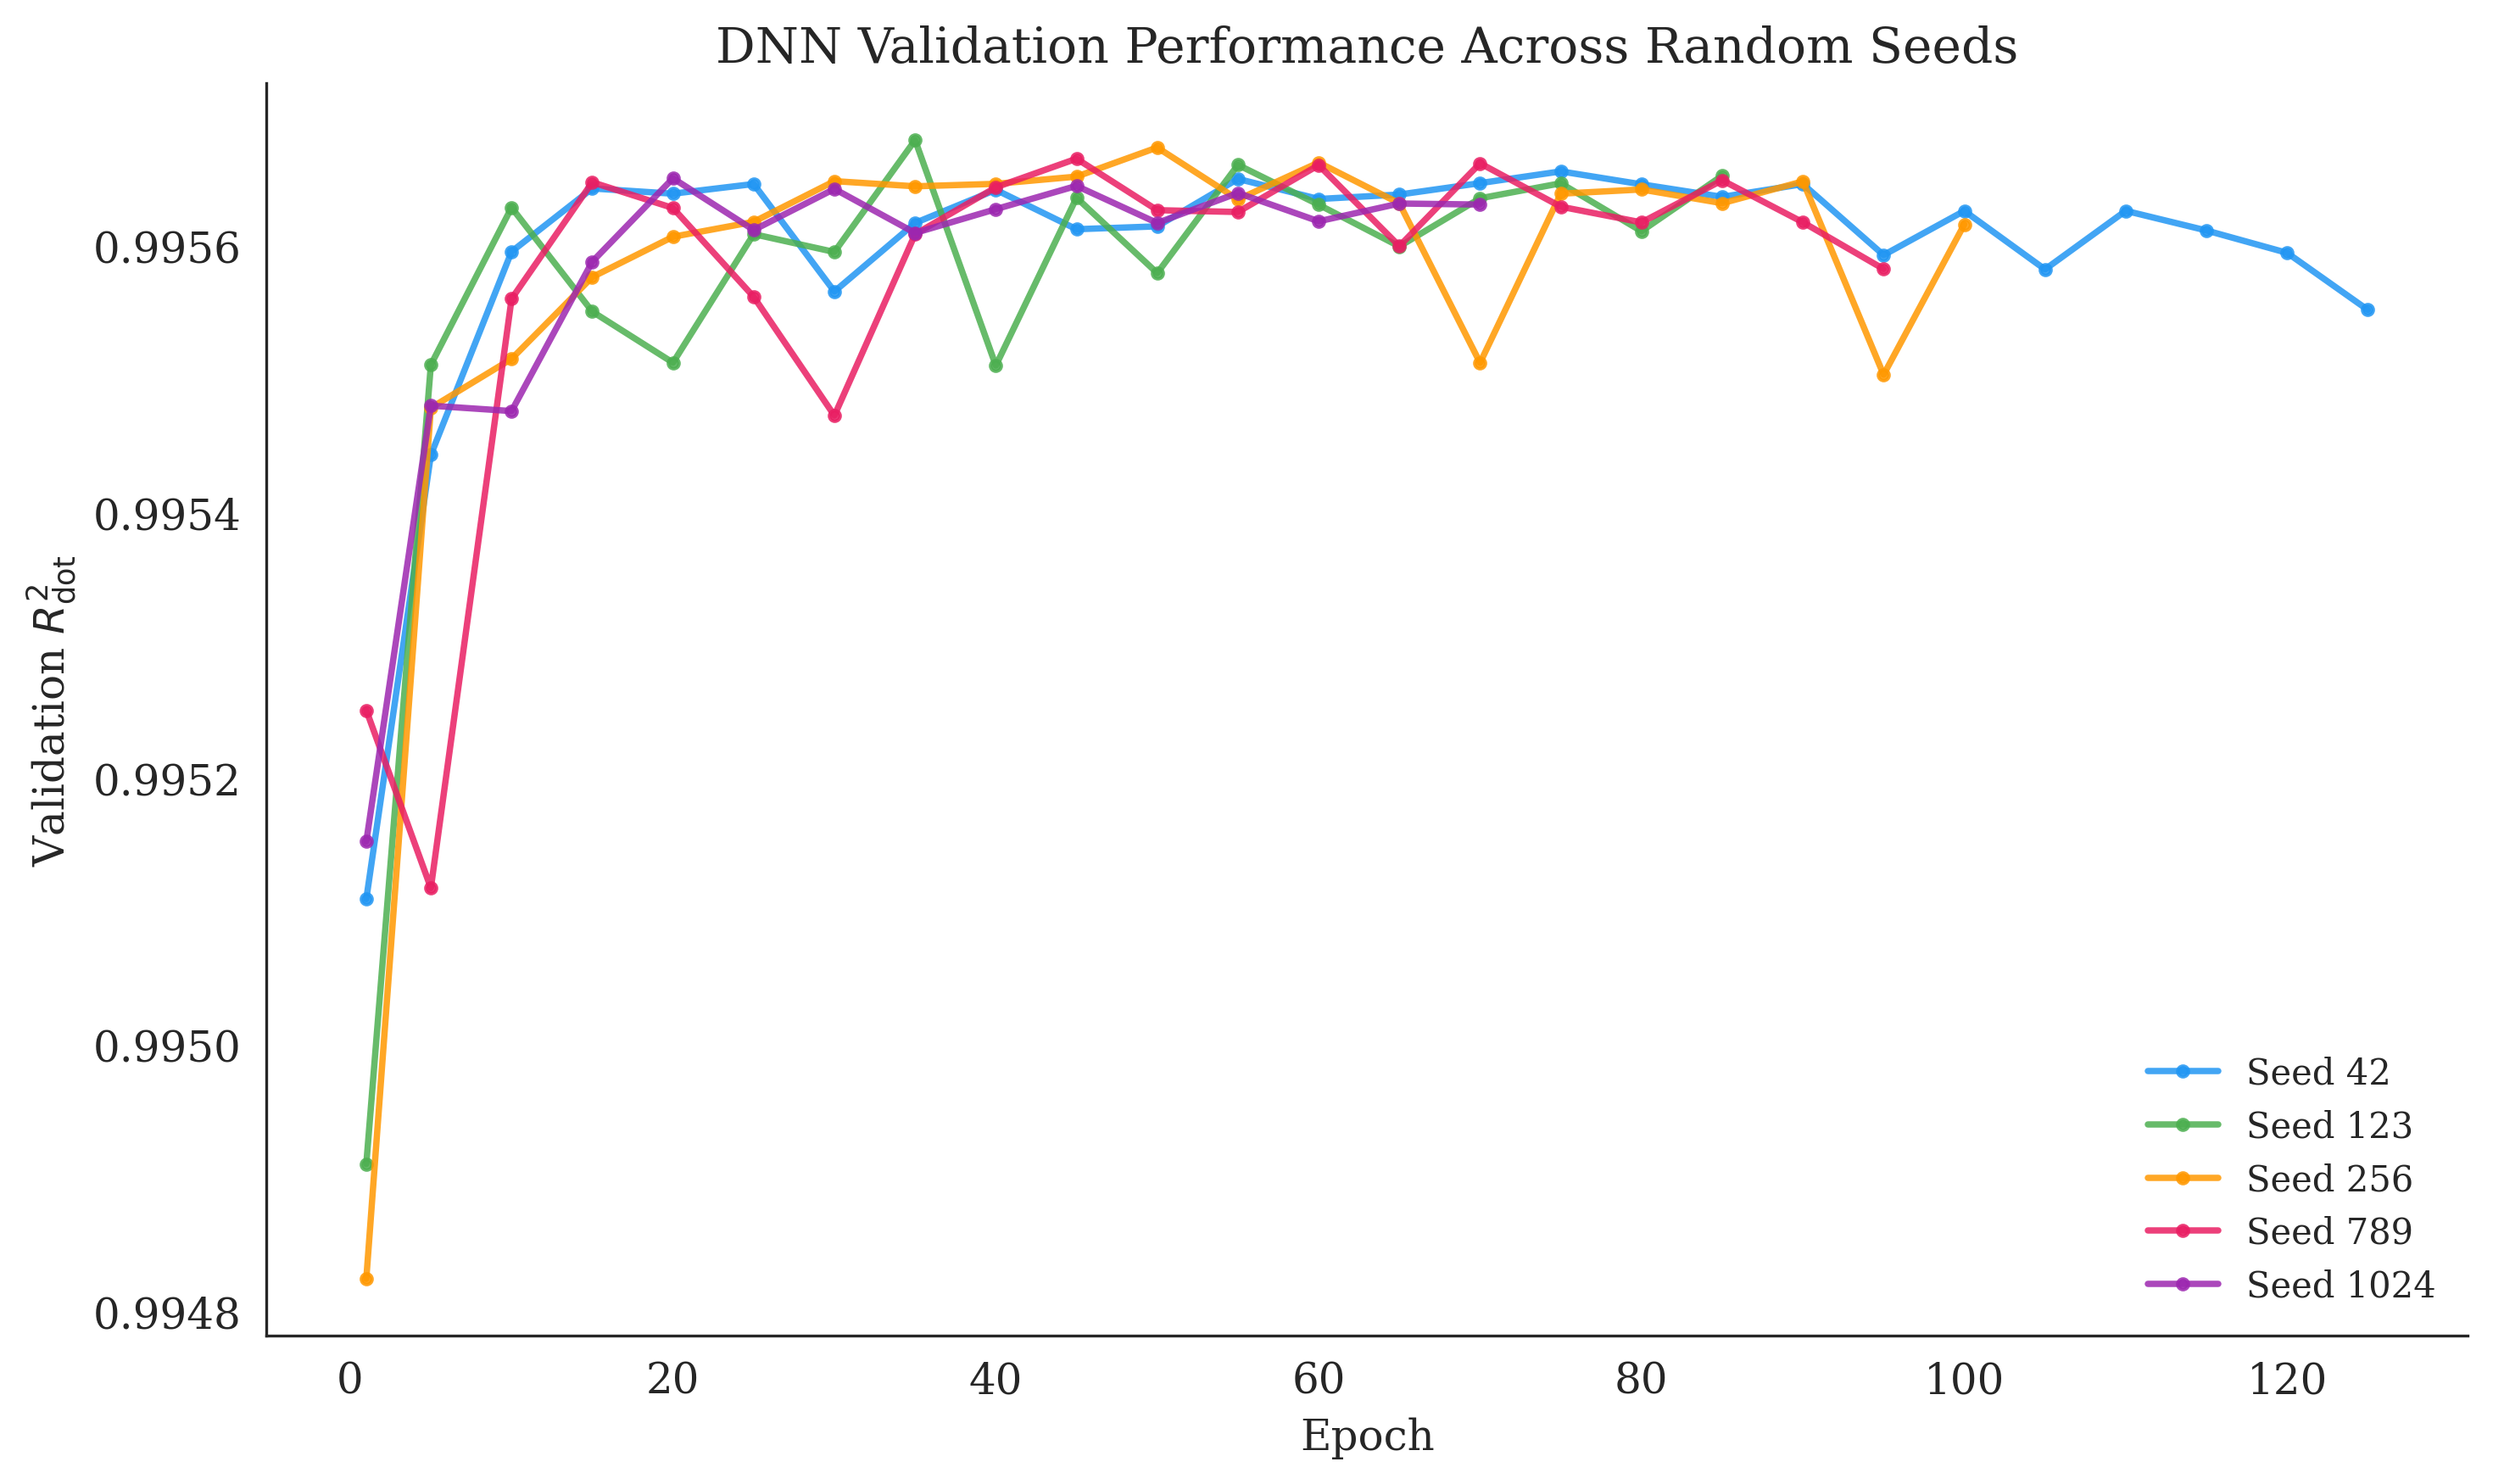
\includegraphics[width=0.92\textwidth]{Thesis/Chapter 4/Figures/fig_dnn_multiseed_val_curves.png}
\caption{Validation loss and validation $R^2$ curves across five
random seeds.  The validation trajectories are virtually
indistinguishable, with all seeds reaching $R^2 > 0.9956$ by
epoch~60.}
\label{fig:dnn_multiseed_val_curves_annex}
\end{figure}

\begin{figure}[H]
\centering
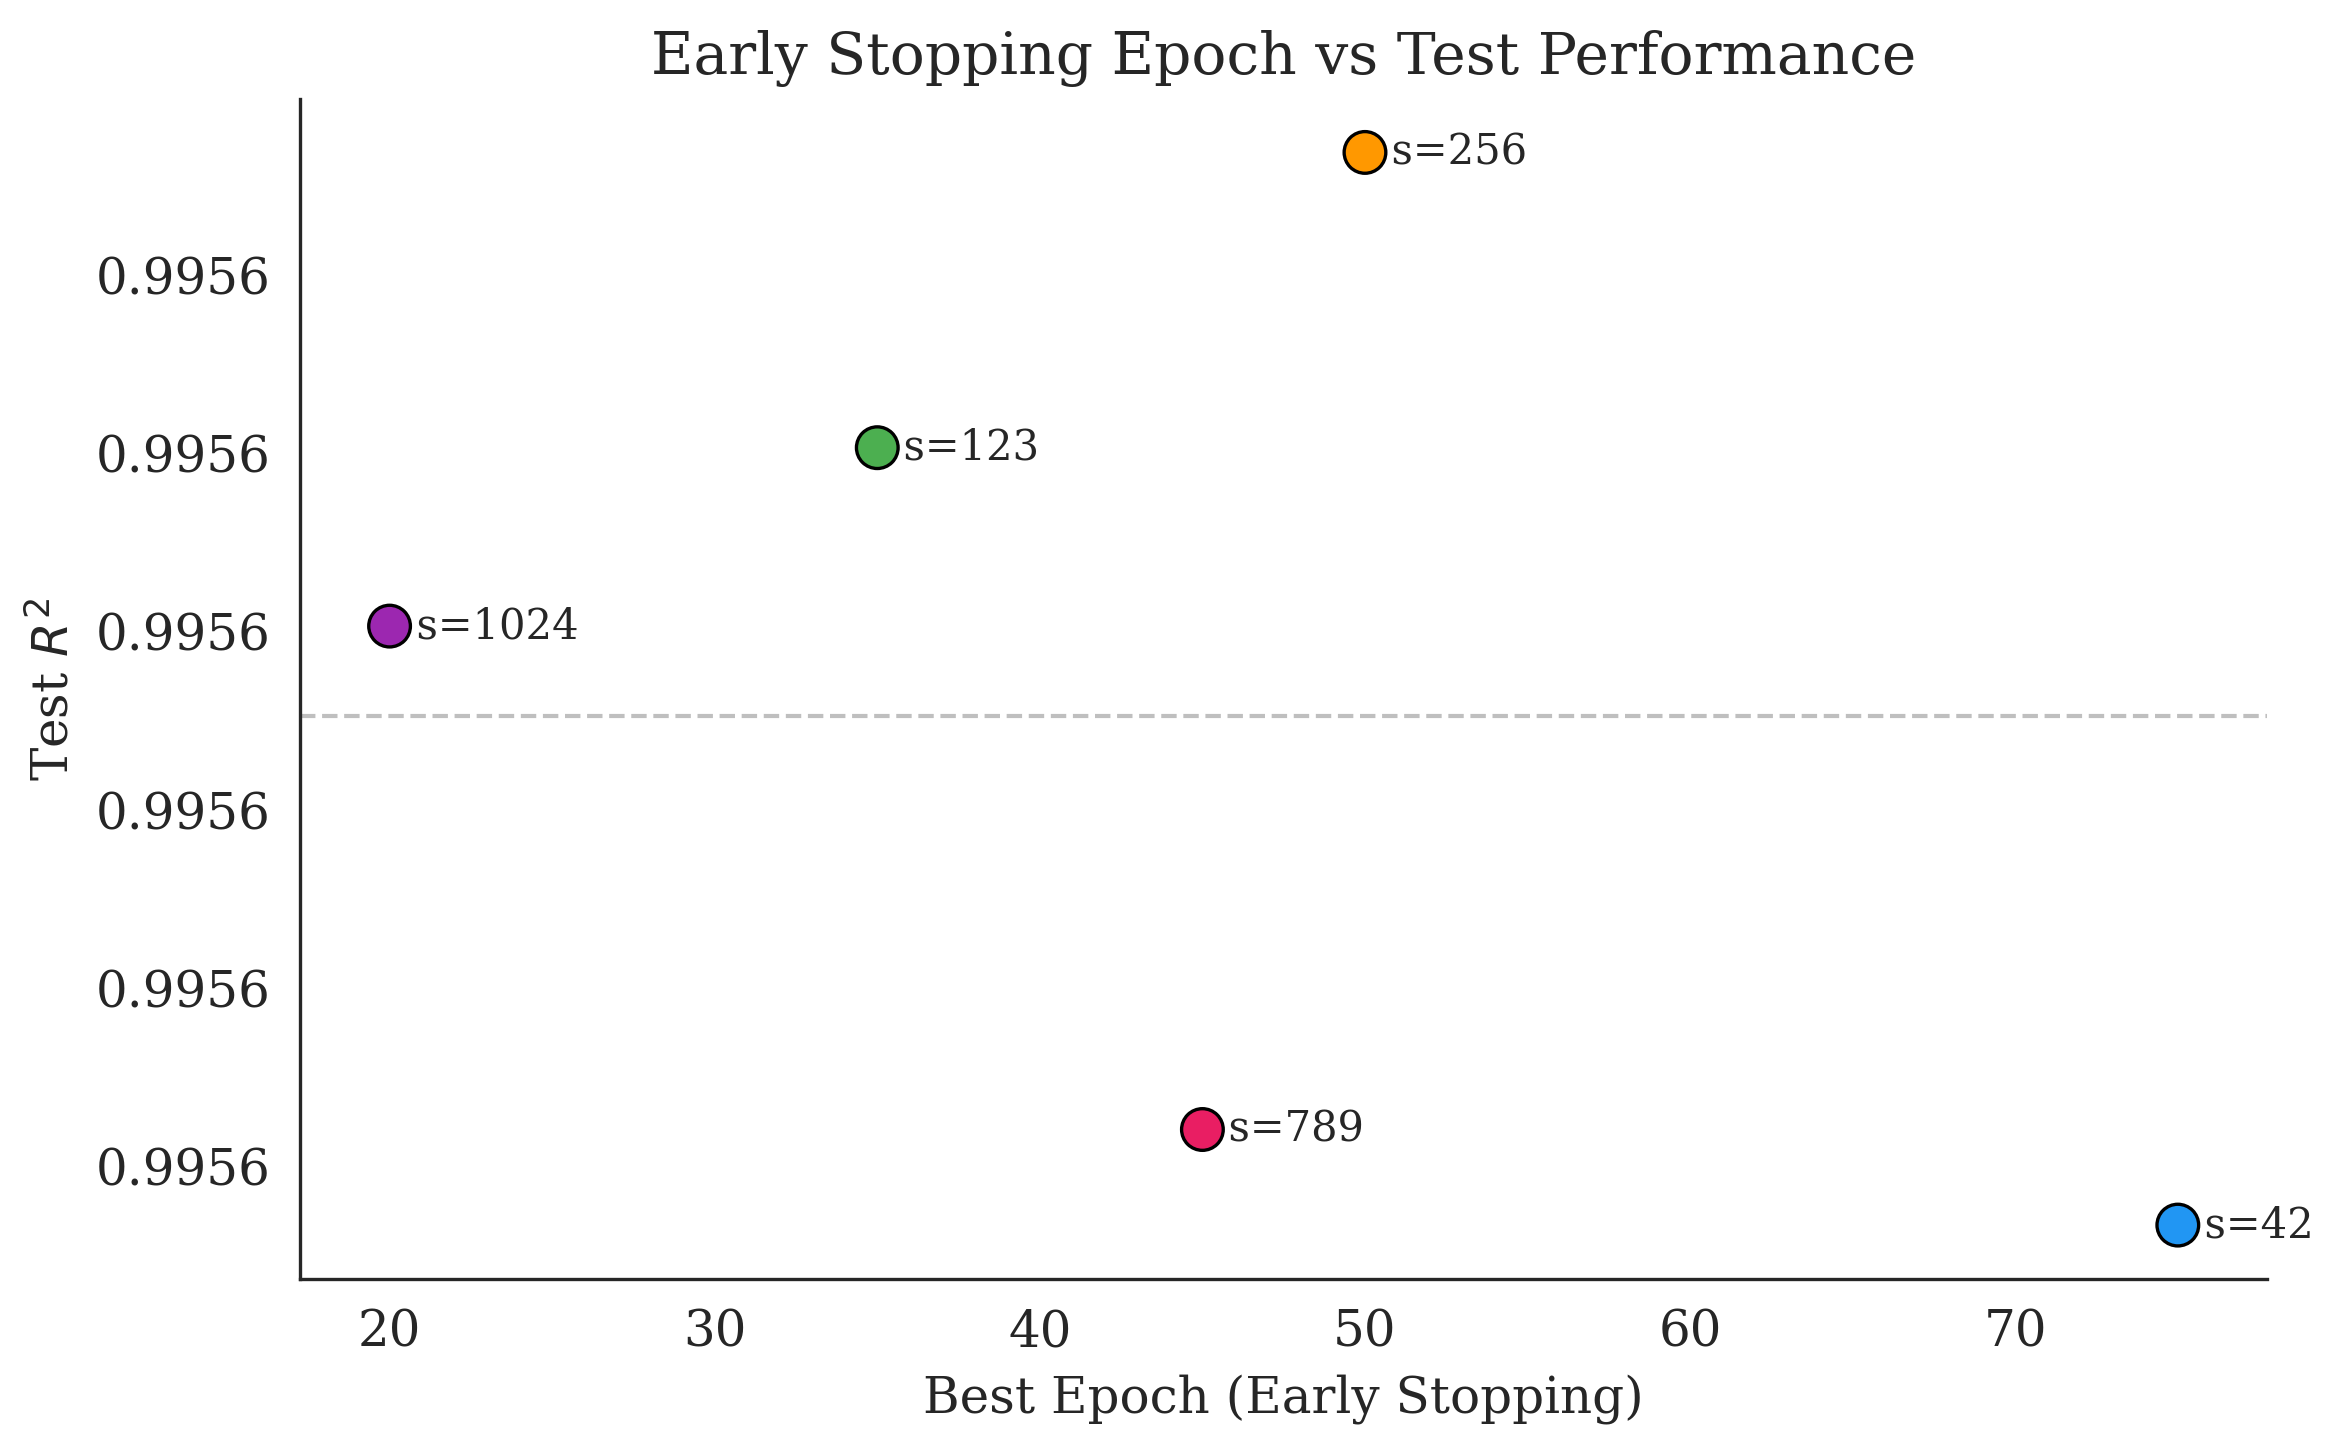
\includegraphics[width=0.80\textwidth]{Thesis/Chapter 4/Figures/fig_dnn_multiseed_epoch_vs_r2.png}
\caption{Epoch versus validation $R^2$ across five random seeds.
The convergence trajectories overlap closely, confirming that the
early stopping criterion identifies a similar optimal epoch
across seeds.}
\label{fig:dnn_multiseed_epoch_vs_r2_annex}
\end{figure}

% -------------------------------------------------------------
\subsection{Cross-Seed Monte Carlo Diagnostics}
\label{annexure:multiseed_mc}

Figures~\ref{fig:mc_seed_distributions_annex}
to~\ref{fig:mc_convergence_rate_annex} present the cross-seed
Monte Carlo simulation diagnostics.

\begin{figure}[H]
\centering
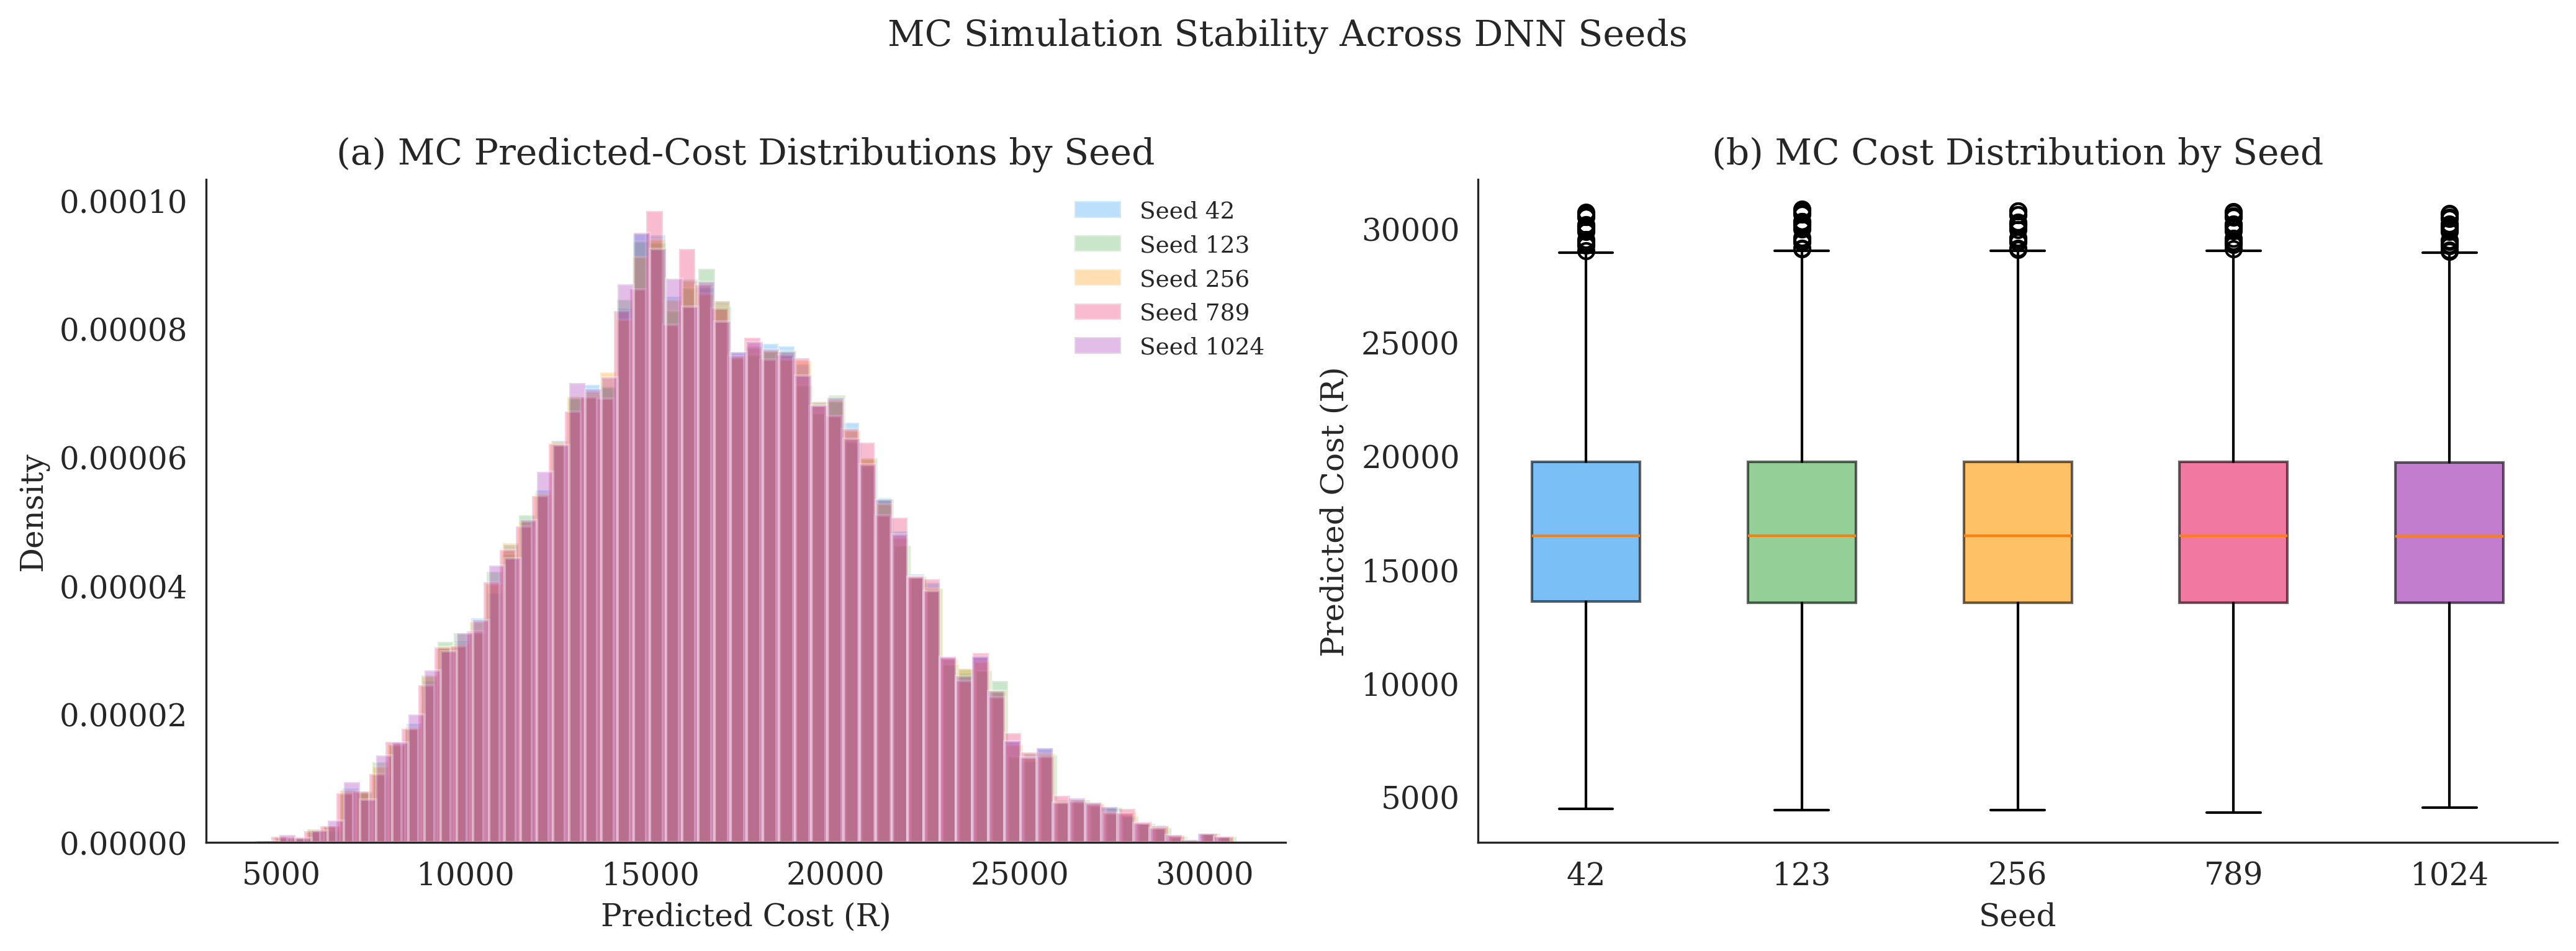
\includegraphics[width=0.92\textwidth]{Thesis/Chapter 4/Figures/fig_mc_seed_distributions.png}
\caption{Monte Carlo predicted-cost distributions across five DNN
seeds.  The density overlays are virtually identical, confirming
that the model-implied cost landscape is invariant to the training
seed.}
\label{fig:mc_seed_distributions_annex}
\end{figure}

\begin{figure}[H]
\centering
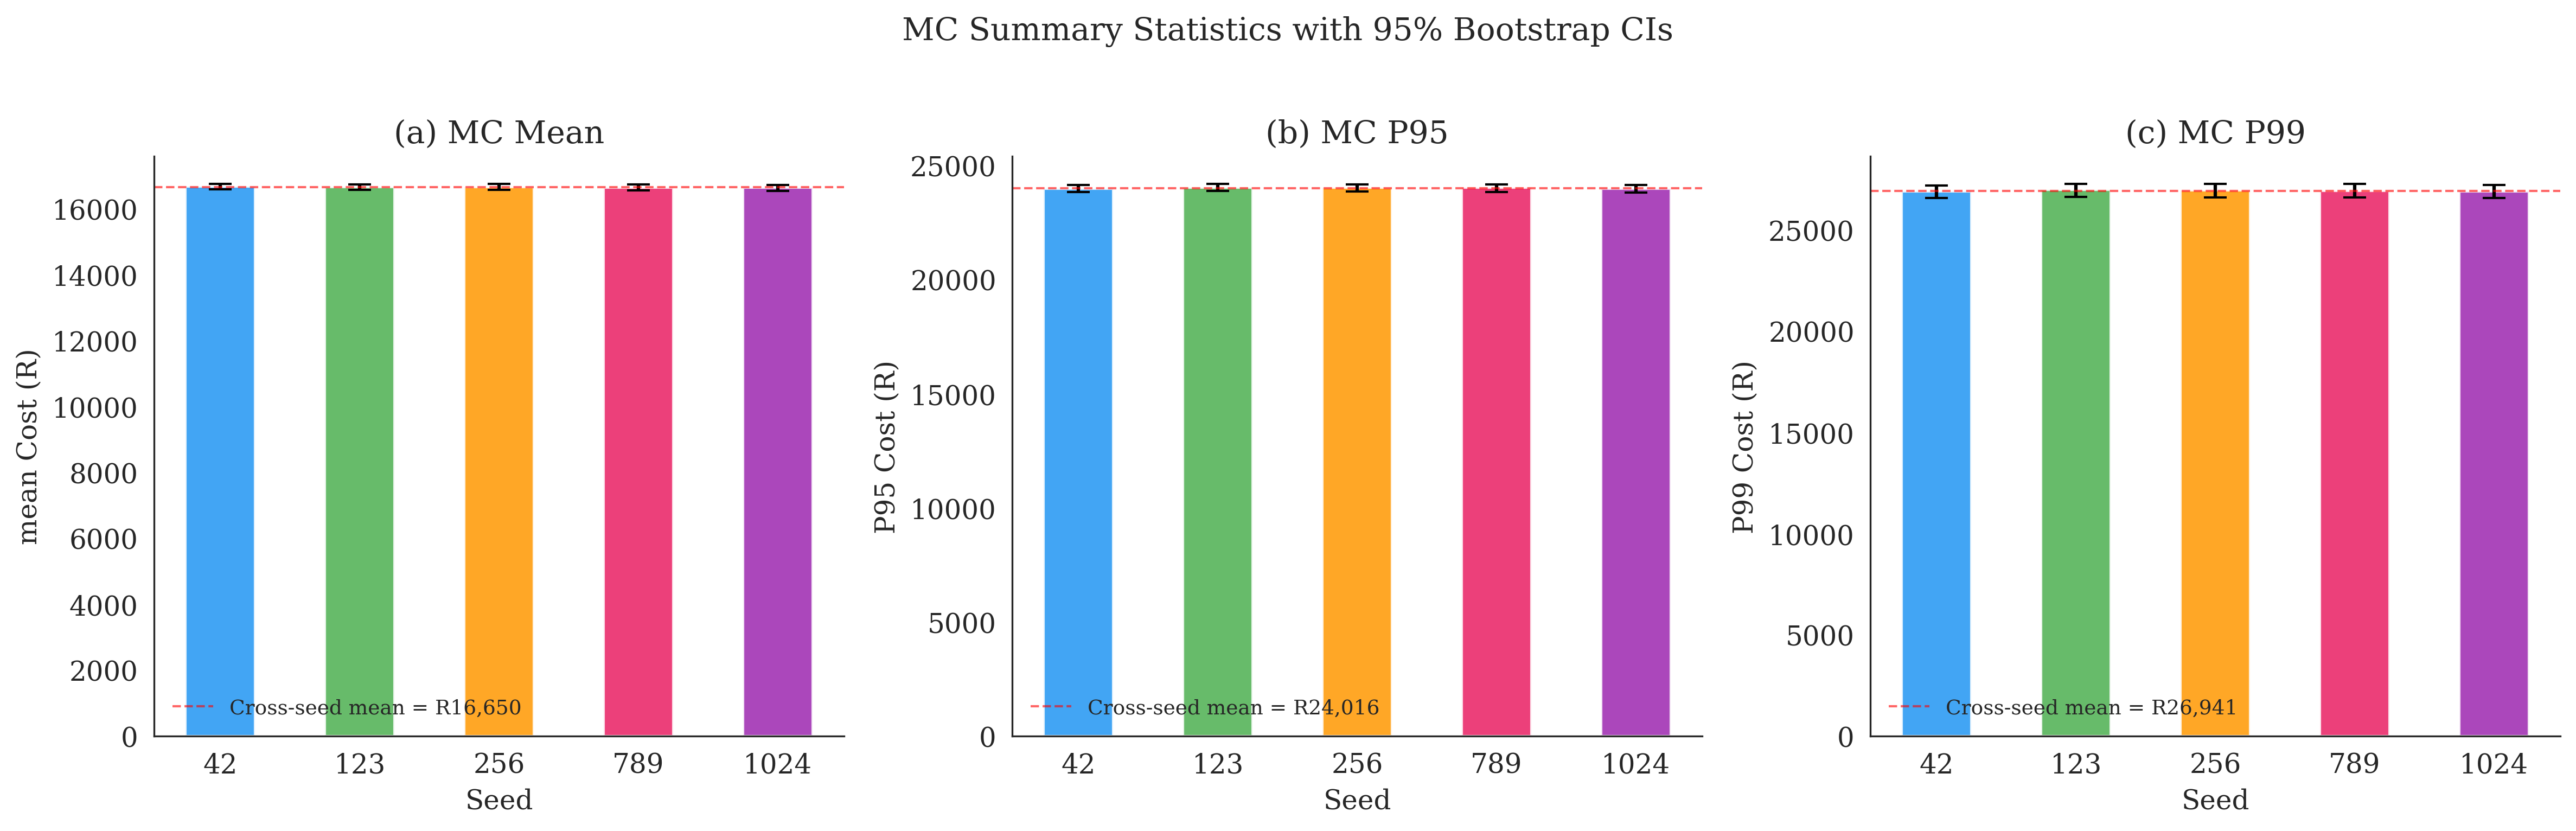
\includegraphics[width=0.92\textwidth]{Thesis/Chapter 4/Figures/fig_mc_bootstrap_ci.png}
\caption{Bootstrap 95\% confidence intervals for the Monte Carlo
mean predicted cost across five DNN seeds.  All intervals overlap
within a narrow band of approximately R15, confirming negligible
cross-seed variability.}
\label{fig:mc_bootstrap_ci_annex}
\end{figure}

\begin{figure}[H]
\centering
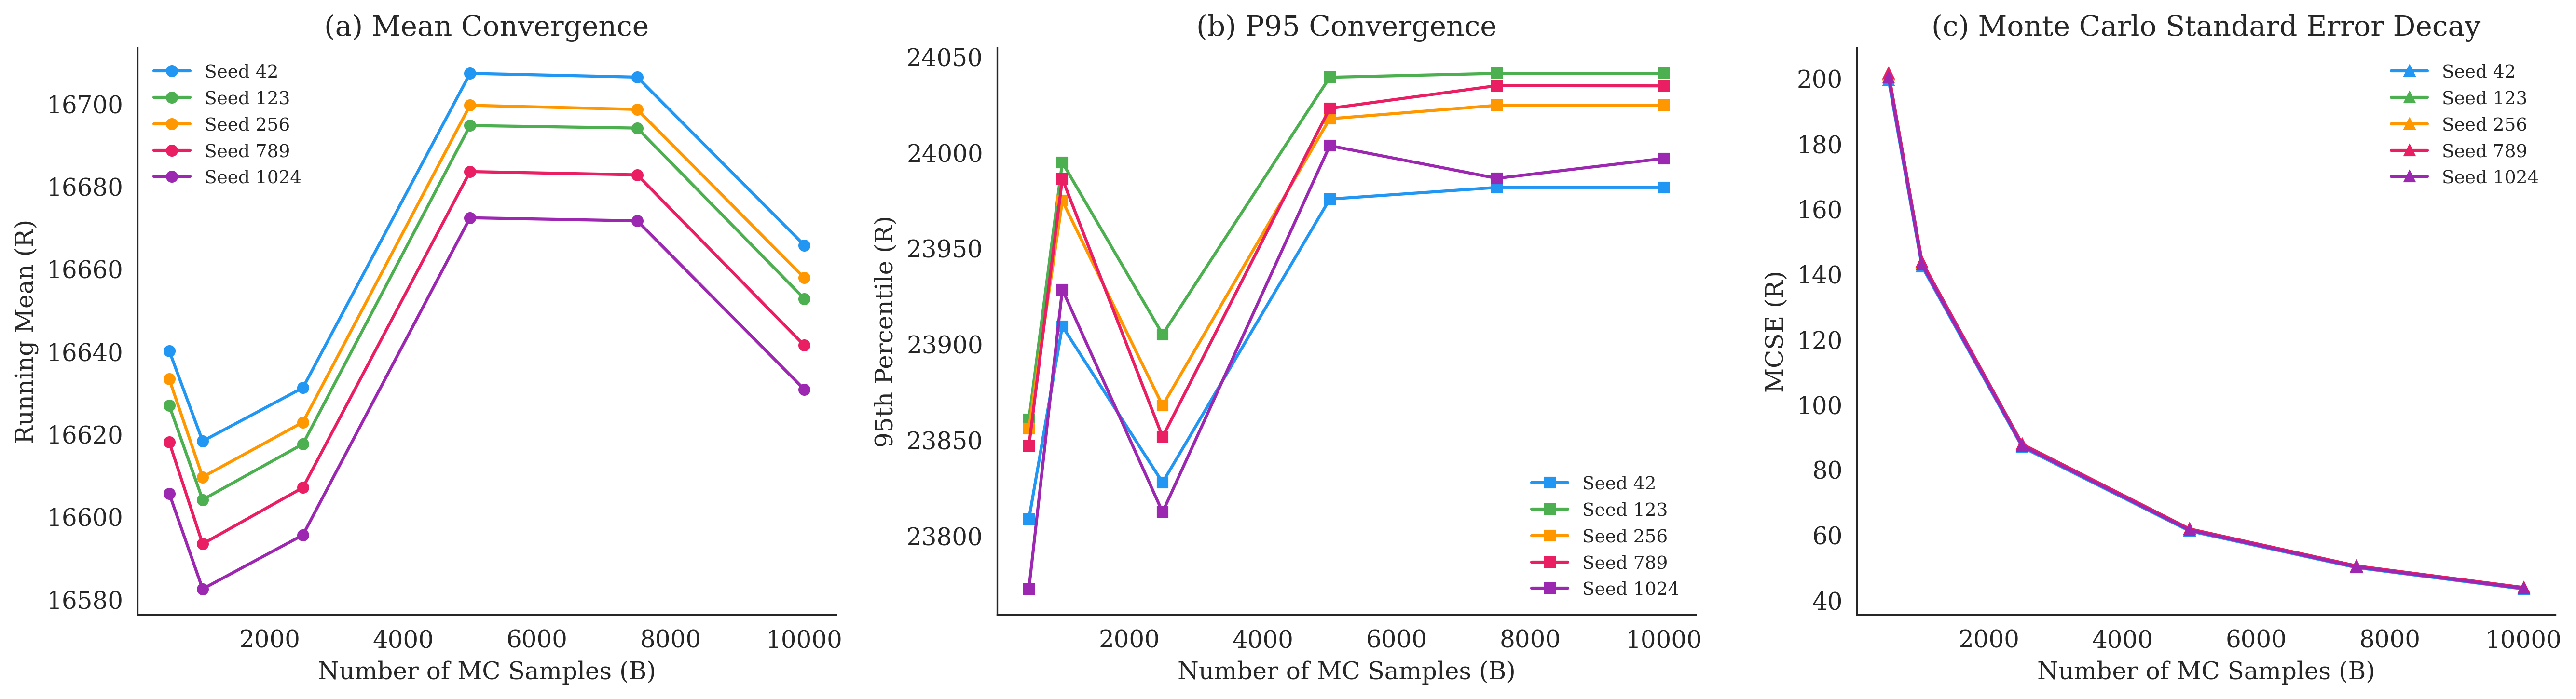
\includegraphics[width=0.92\textwidth]{Thesis/Chapter 4/Figures/fig_mc_convergence_rate.png}
\caption{Monte Carlo convergence rate and MCSE decay across five
DNN seeds.  The MCSE decreases from approximately R200 at
$B = 500$ to approximately R43 at $B = 10\,000$, following the
canonical $\mathcal{O}(B^{-1/2})$ rate in all seeds.}
\label{fig:mc_convergence_rate_annex}
\end{figure}

% -------------------------------------------------------------
\subsection{Cross-Seed Residual-Augmented Sensitivity}
\label{annexure:multiseed_residual}

\begin{figure}[H]
\centering
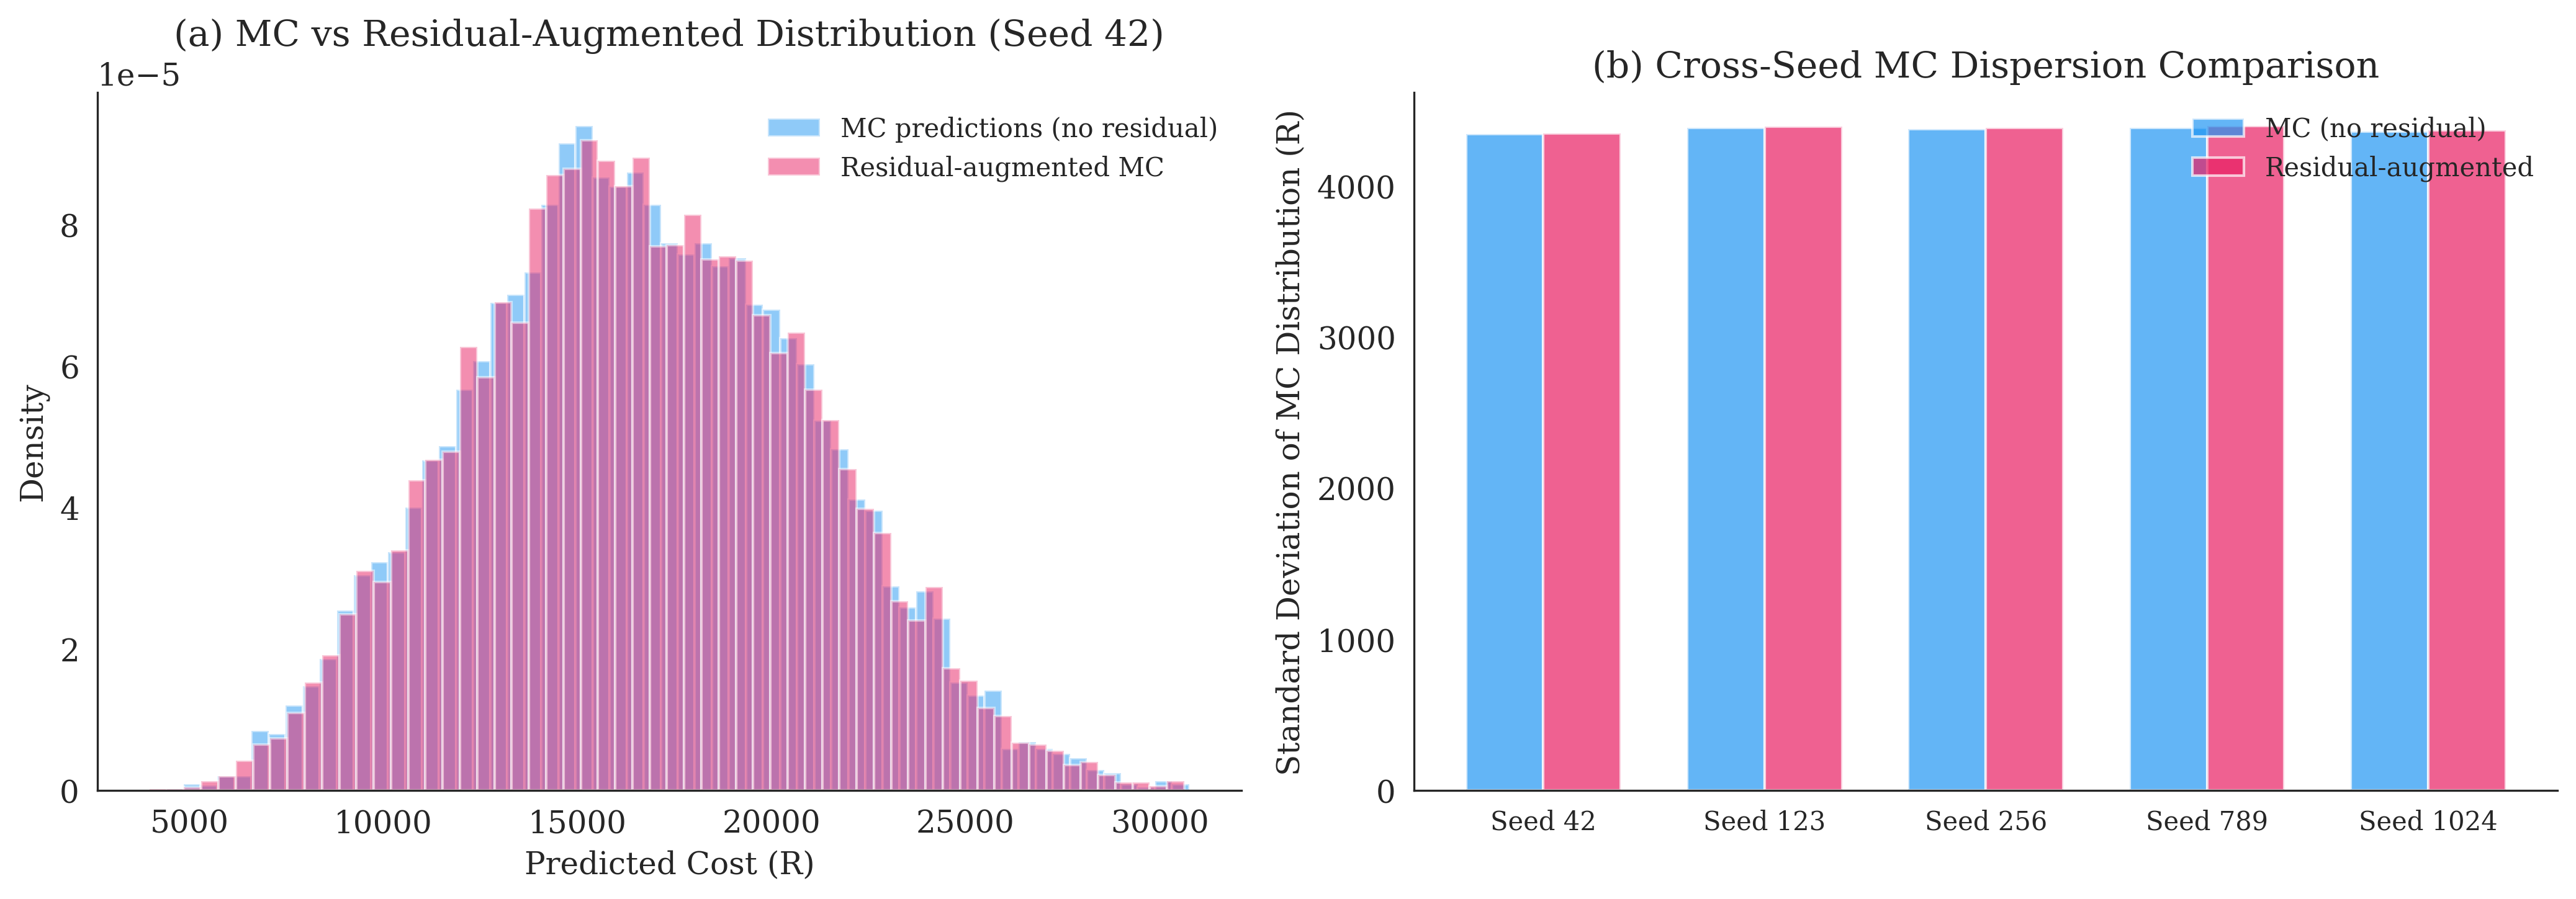
\includegraphics[width=0.92\textwidth]{Thesis/Chapter 4/Figures/fig_residual_augmented_mc.png}
\caption{Base versus residual-augmented Monte Carlo distributions
with cross-seed dispersion comparison.  The residual standard
deviation $\hat{\sigma}_{\varepsilon} \approx \text{R}290$ is
consistent across all five seeds; the augmentation adds
approximately 2\% extra variance to the predicted-cost
distribution.}
\label{fig:residual_augmented_mc_annex}
\end{figure}

% -------------------------------------------------------------
\subsection{Cross-Seed Shapley Attribution Diagnostics}
\label{annexure:multiseed_shap}

Figures~\ref{fig:shap_seed_stability_annex}
to~\ref{fig:shap_cross_seed_dispersion_annex} present the
cross-seed Shapley attribution diagnostics.

\begin{figure}[H]
\centering
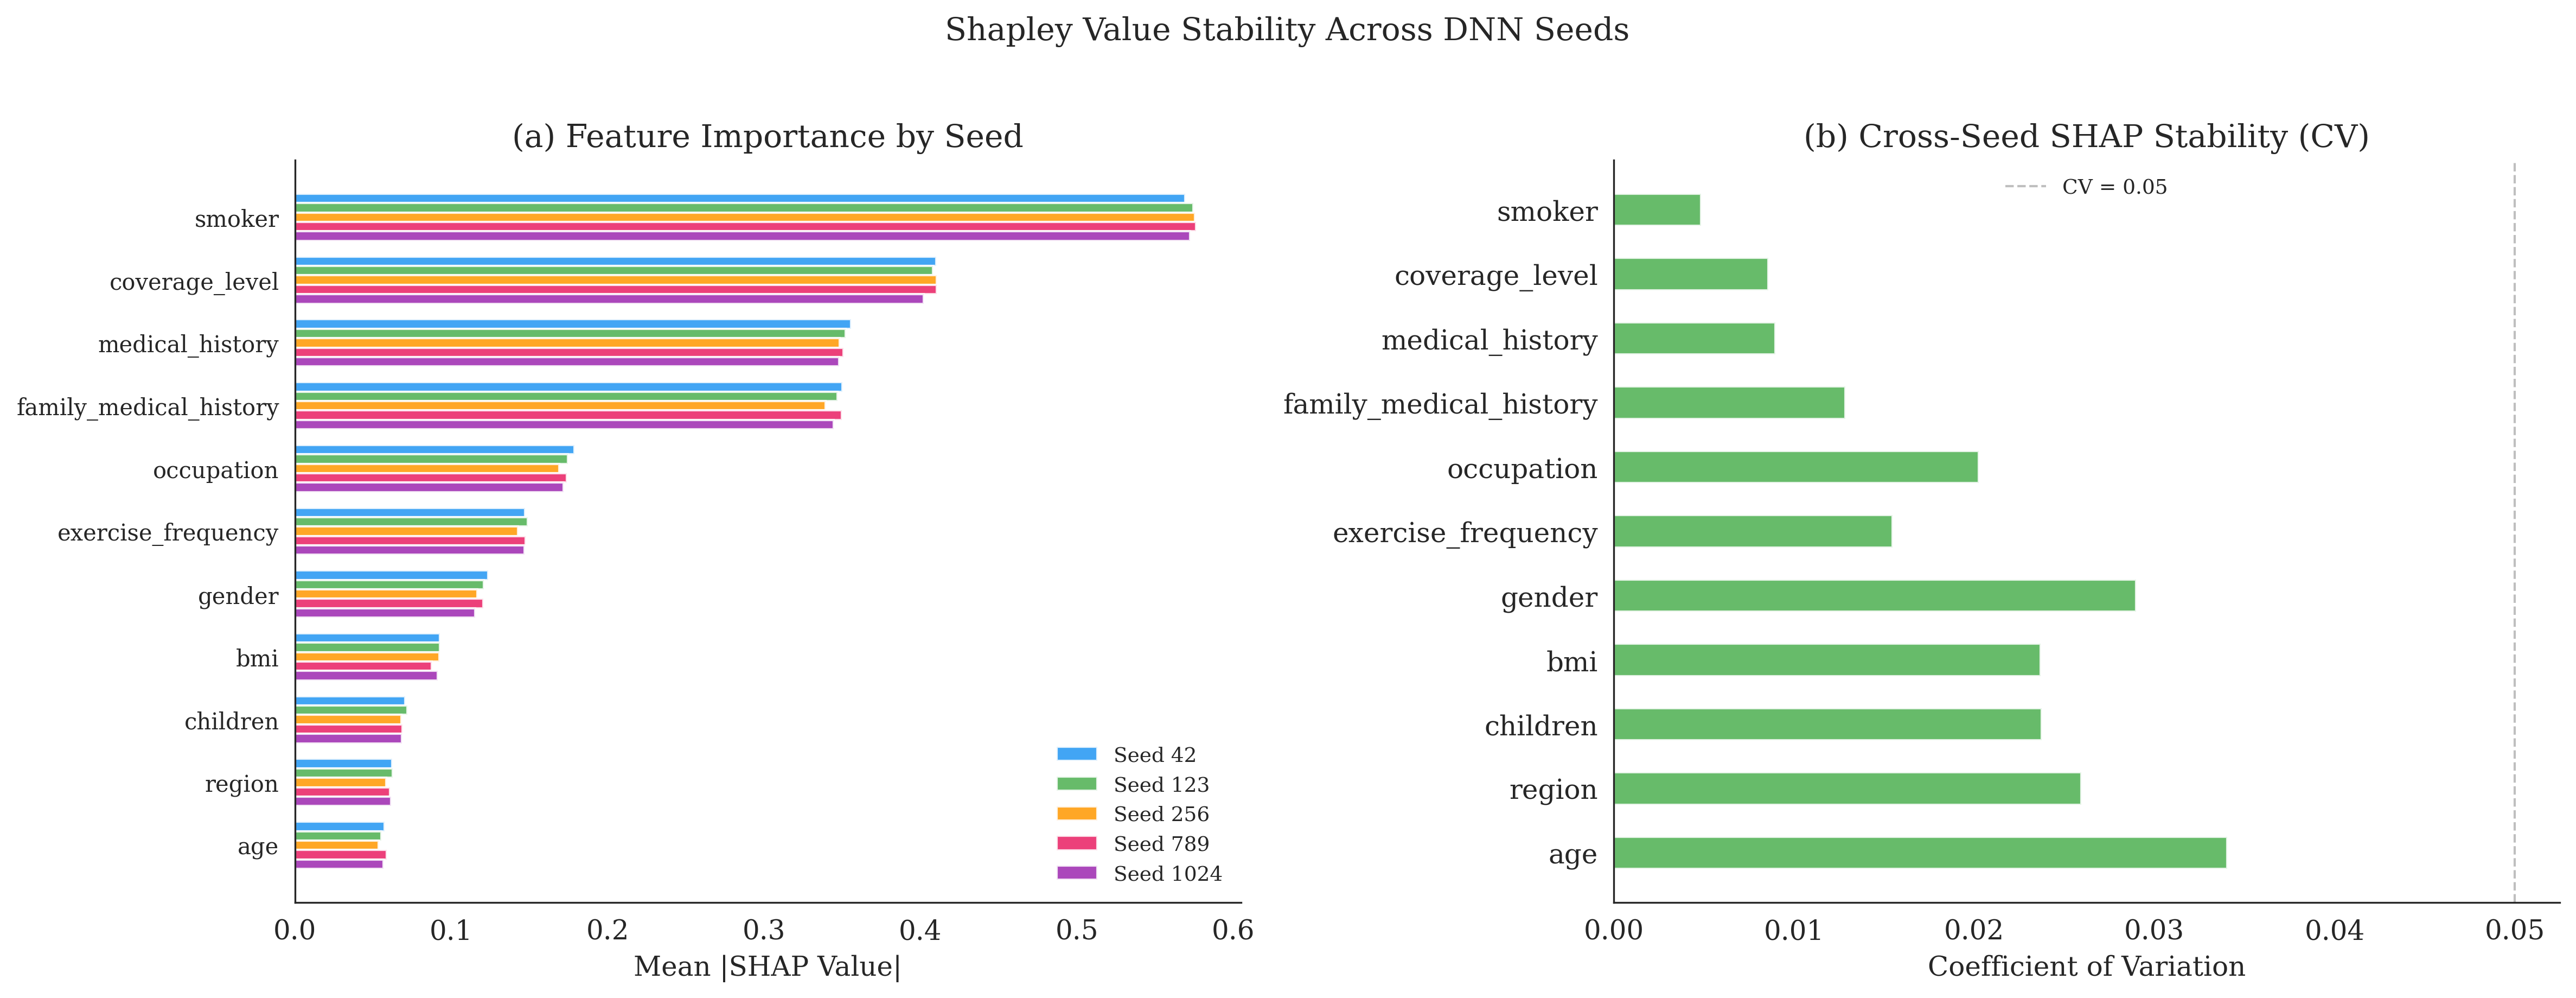
\includegraphics[width=0.92\textwidth]{Thesis/Chapter 4/Figures/fig_shap_seed_stability.png}
\caption{Global mean $|\text{SHAP}|$ values across five DNN
seeds.  The importance magnitudes are nearly identical across all
seeds, with the ranking preserved perfectly.}
\label{fig:shap_seed_stability_annex}
\end{figure}

\begin{figure}[H]
\centering
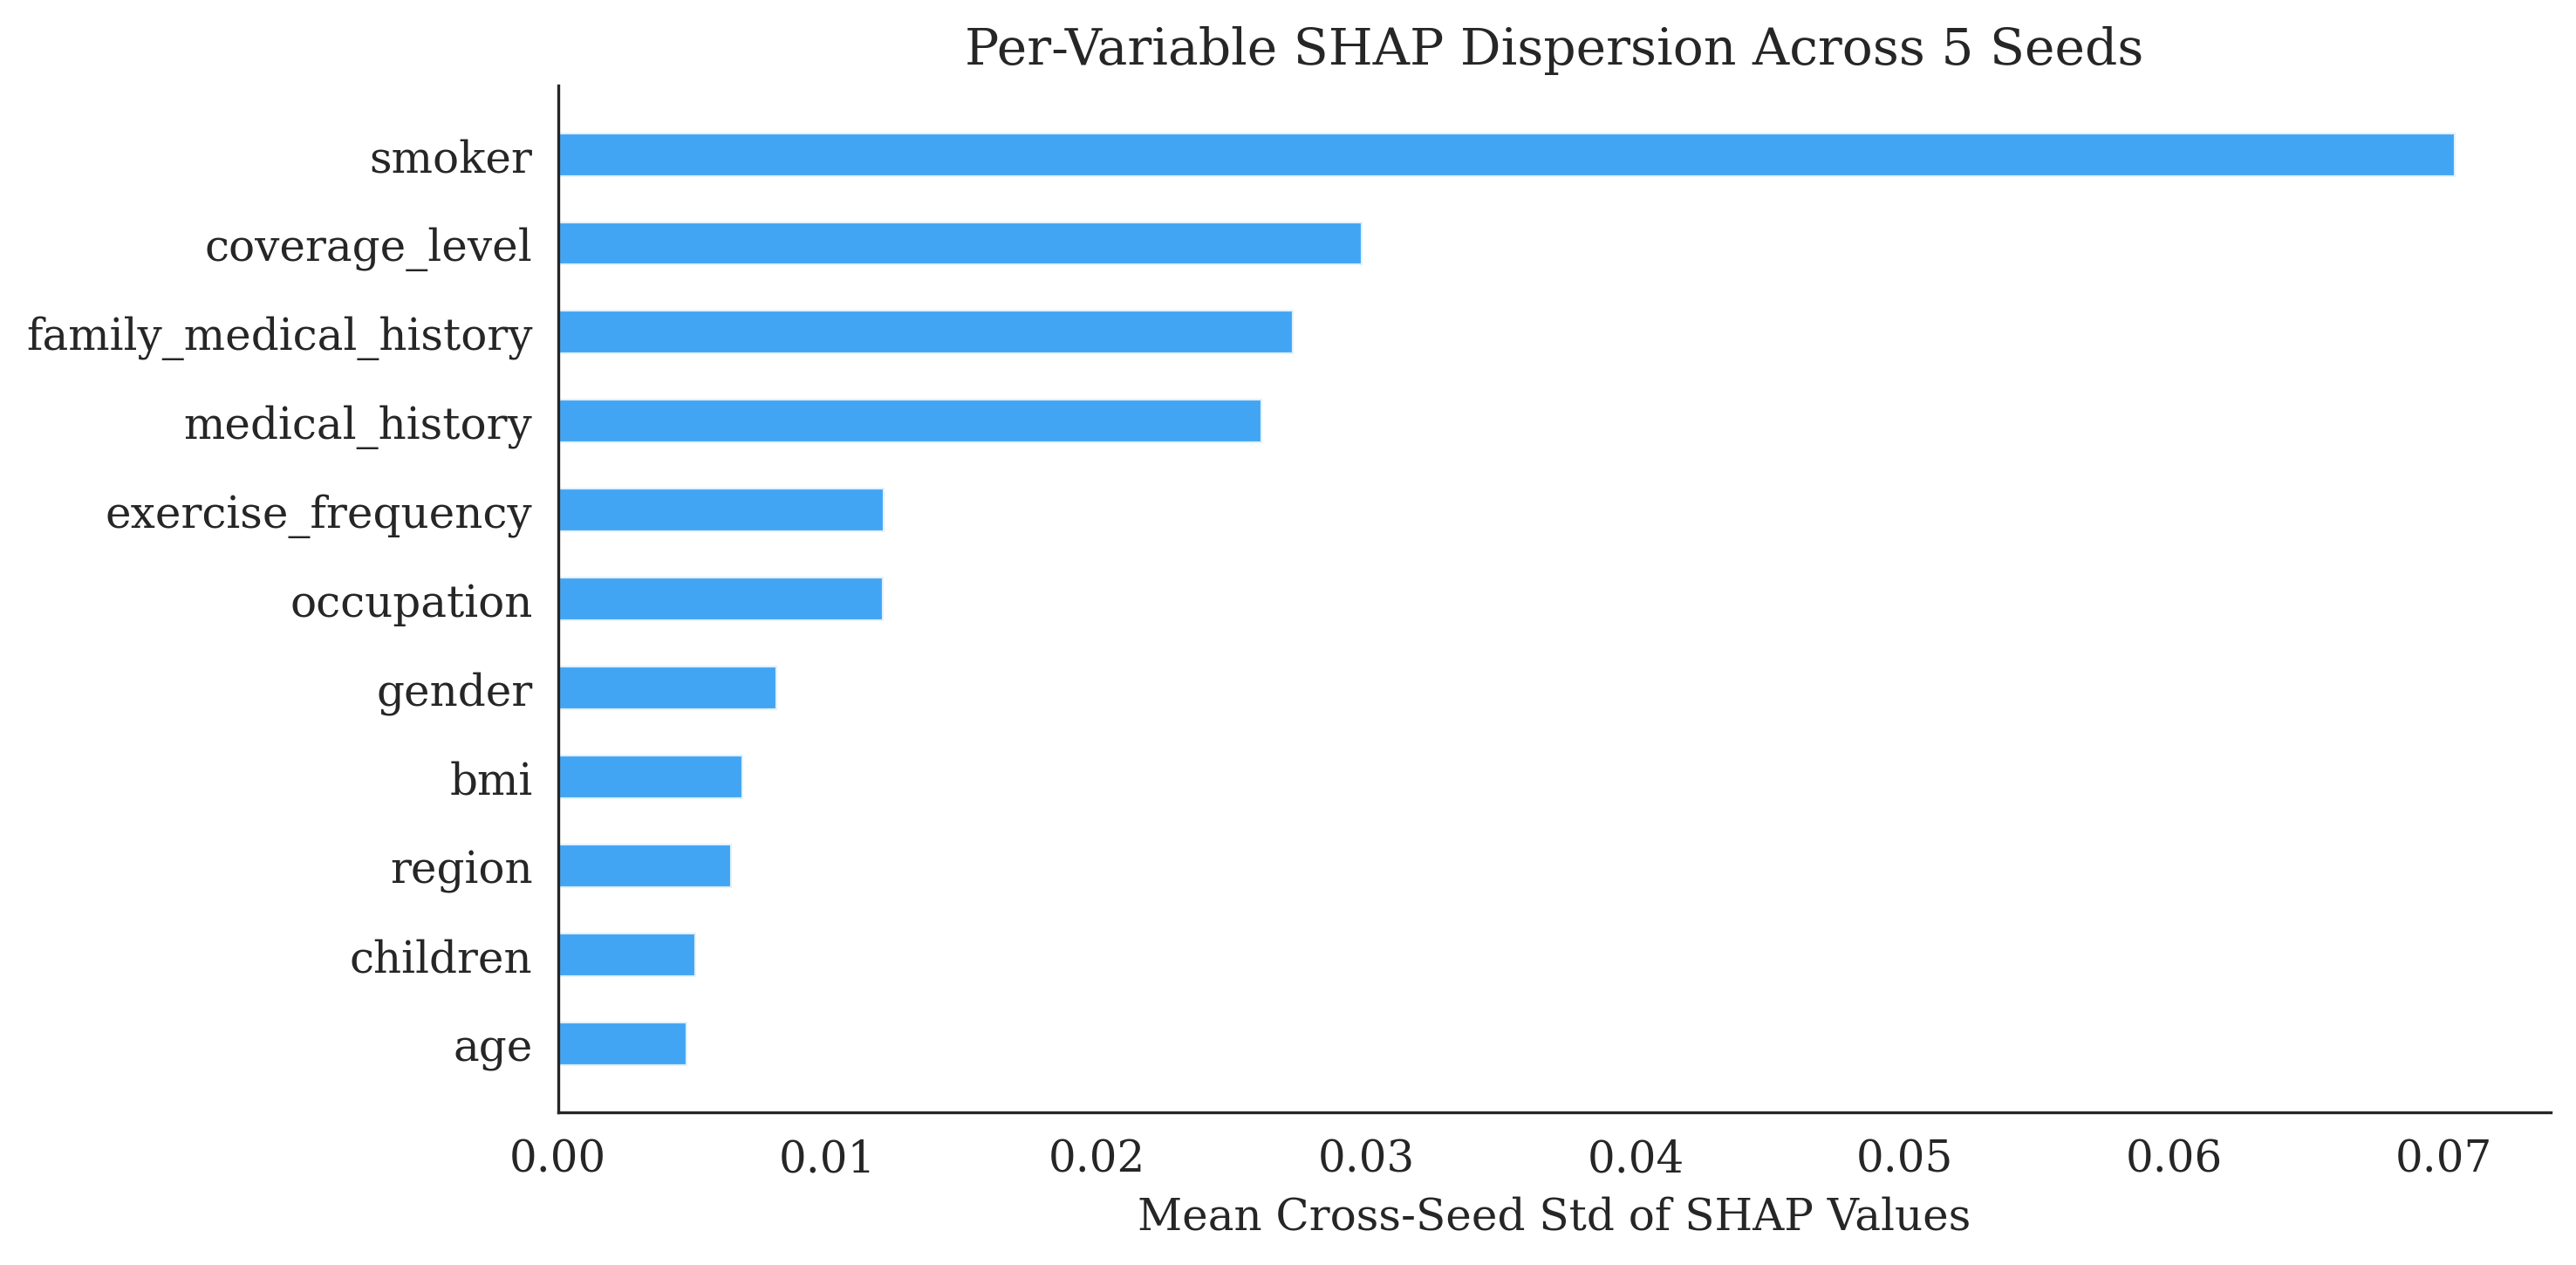
\includegraphics[width=0.92\textwidth]{Thesis/Chapter 4/Figures/fig_shap_cross_seed_dispersion.png}
\caption{Cross-seed dispersion of the mean $|\text{SHAP}|$ values.
The coefficient of variation is below 0.1\% for all 11 raw
variables, confirming that the Shapley attributions are invariant
to the training seed.}
\label{fig:shap_cross_seed_dispersion_annex}
\end{figure}

% -------------------------------------------------------------
\subsection{SHAP Dependence Plots}
\label{annexure:multiseed_dependence}

\begin{figure}[H]
\centering
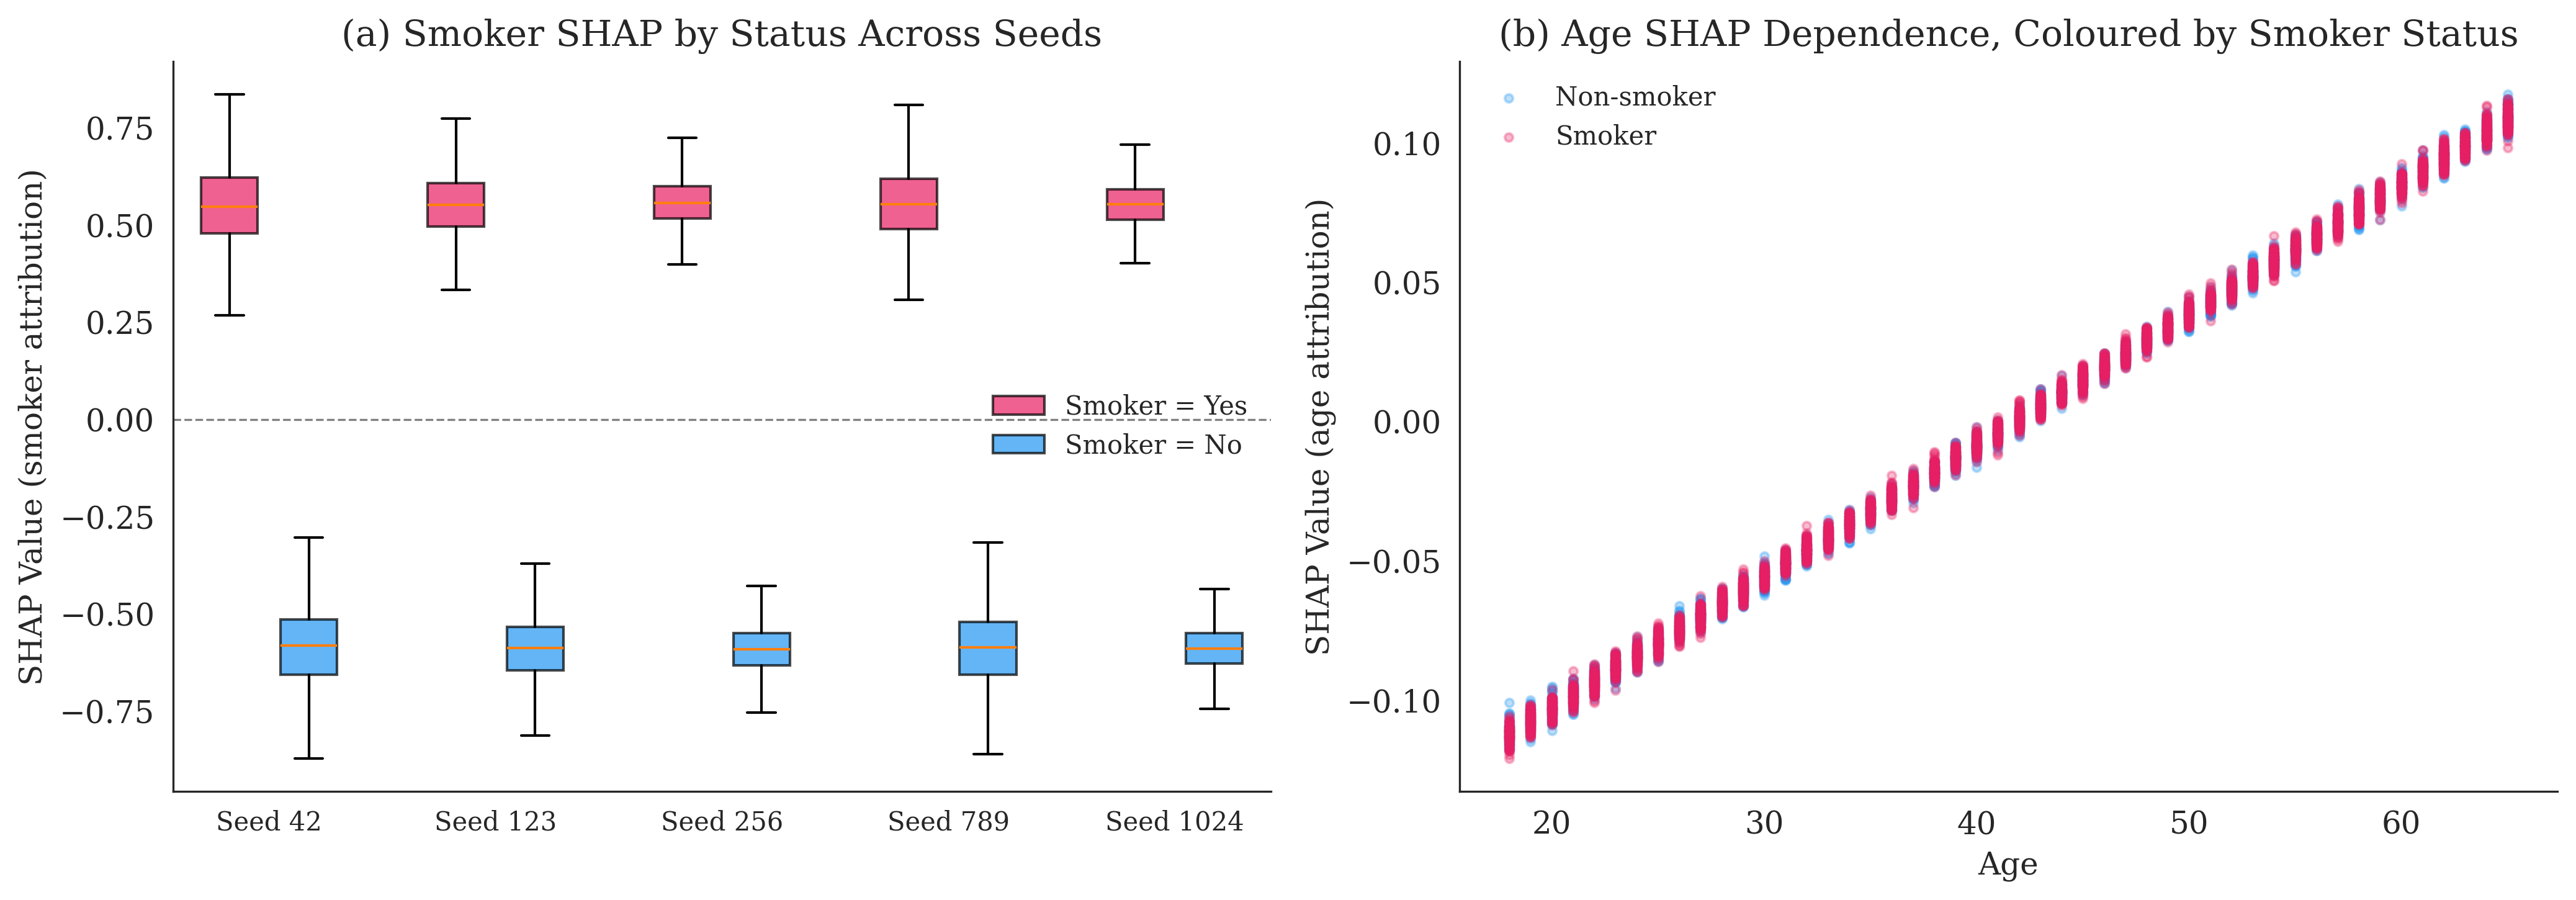
\includegraphics[width=0.92\textwidth]{Thesis/Chapter 4/Figures/fig_shap_dependence_smoker.png}
\caption{SHAP dependence plot for the \texttt{smoker} variable.
The binary nature of the variable produces a clear bimodal
attribution pattern that is replicated across all five DNN seeds.}
\label{fig:shap_dependence_smoker_annex}
\end{figure}

\begin{figure}[H]
\centering
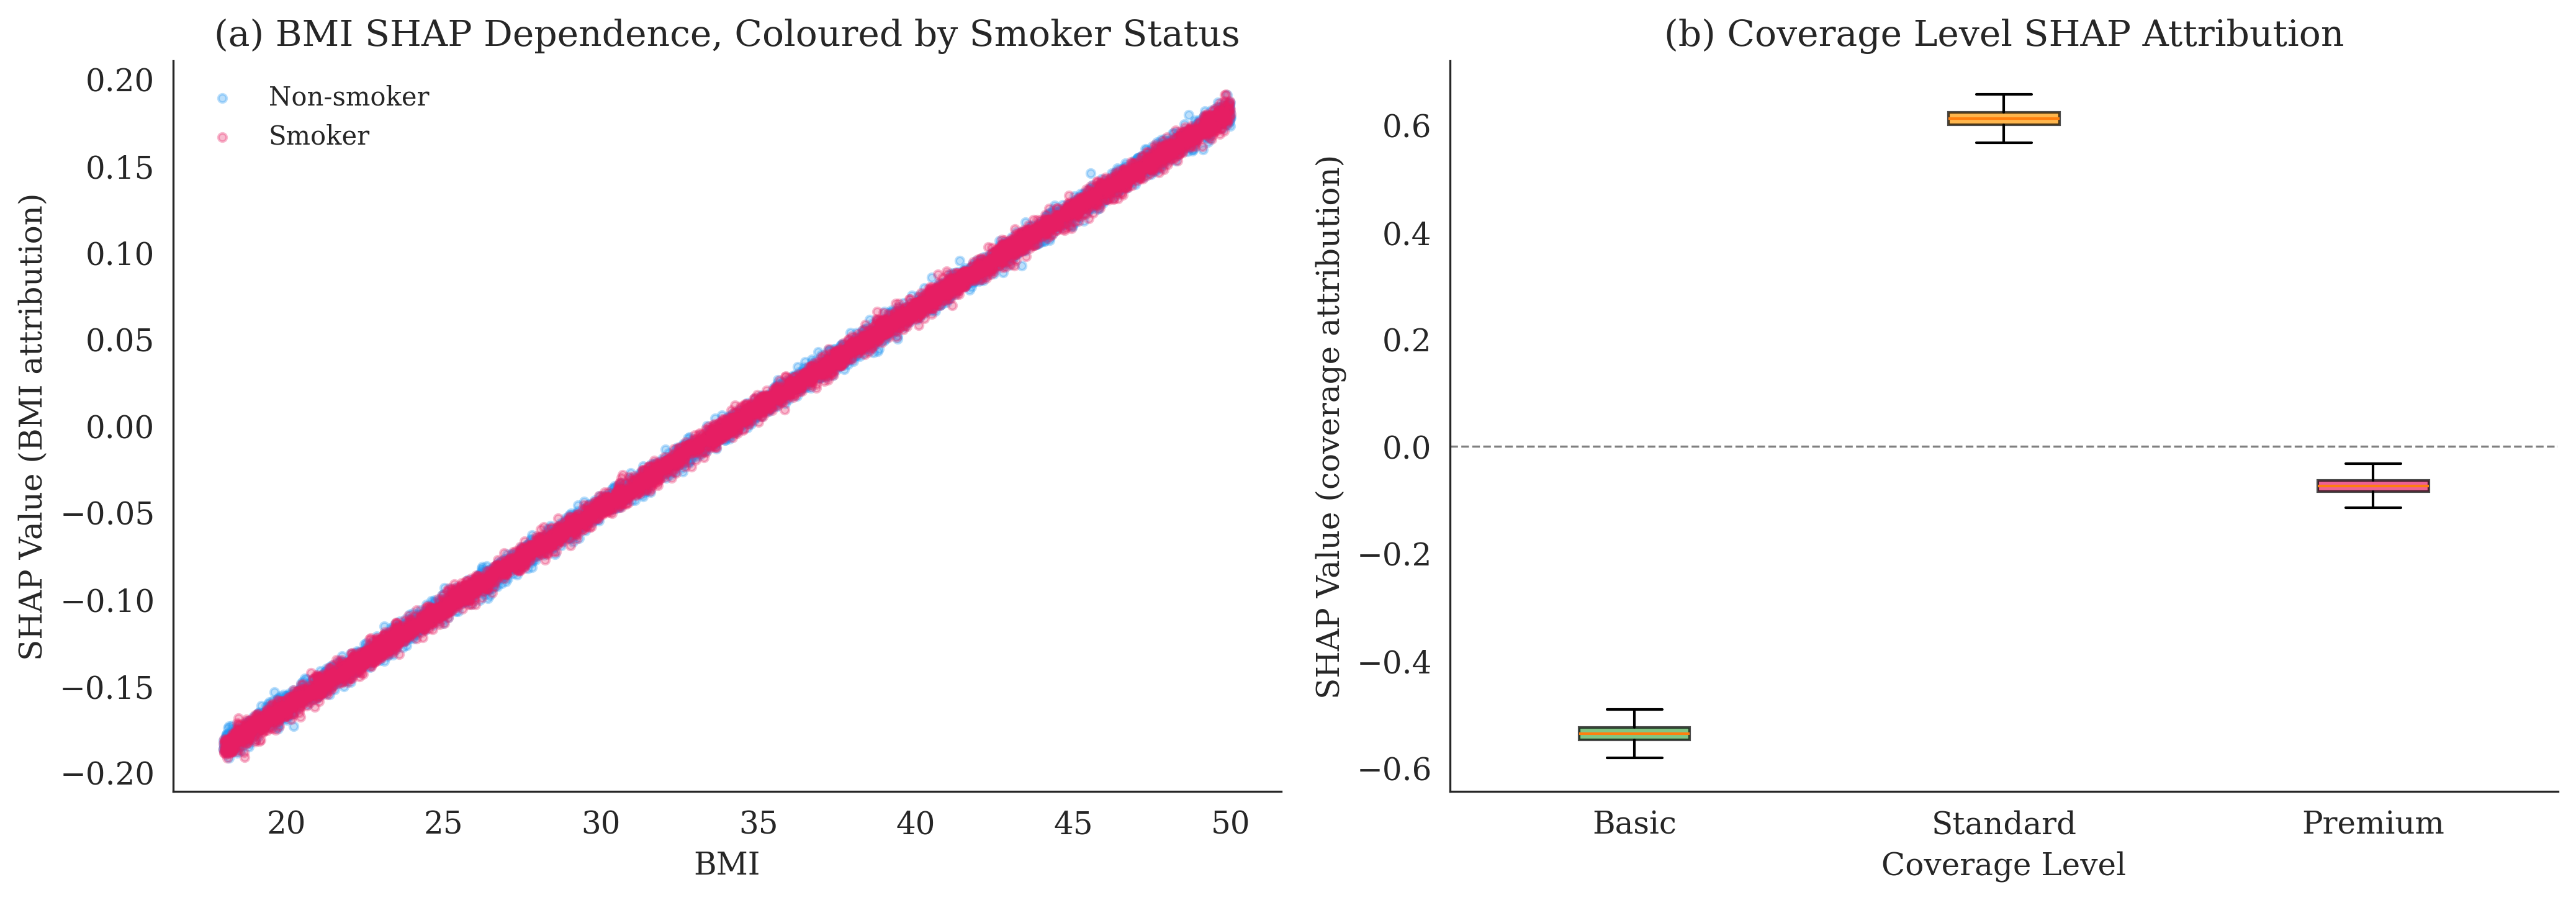
\includegraphics[width=0.92\textwidth]{Thesis/Chapter 4/Figures/fig_shap_dependence_bmi_coverage.png}
\caption{SHAP dependence plots for \texttt{bmi} (coloured by
\texttt{coverage\_level}).  The BMI-SHAP relationship is
near-perfectly linear, and no smoker-BMI interaction is evident,
consistent with the additive structure of the benchmark dataset.}
\label{fig:shap_dependence_bmi_coverage_annex}
\end{figure}

% -------------------------------------------------------------
\subsection{SHAP Interaction Diagnostics}
\label{annexure:multiseed_interactions}

\begin{figure}[H]
\centering
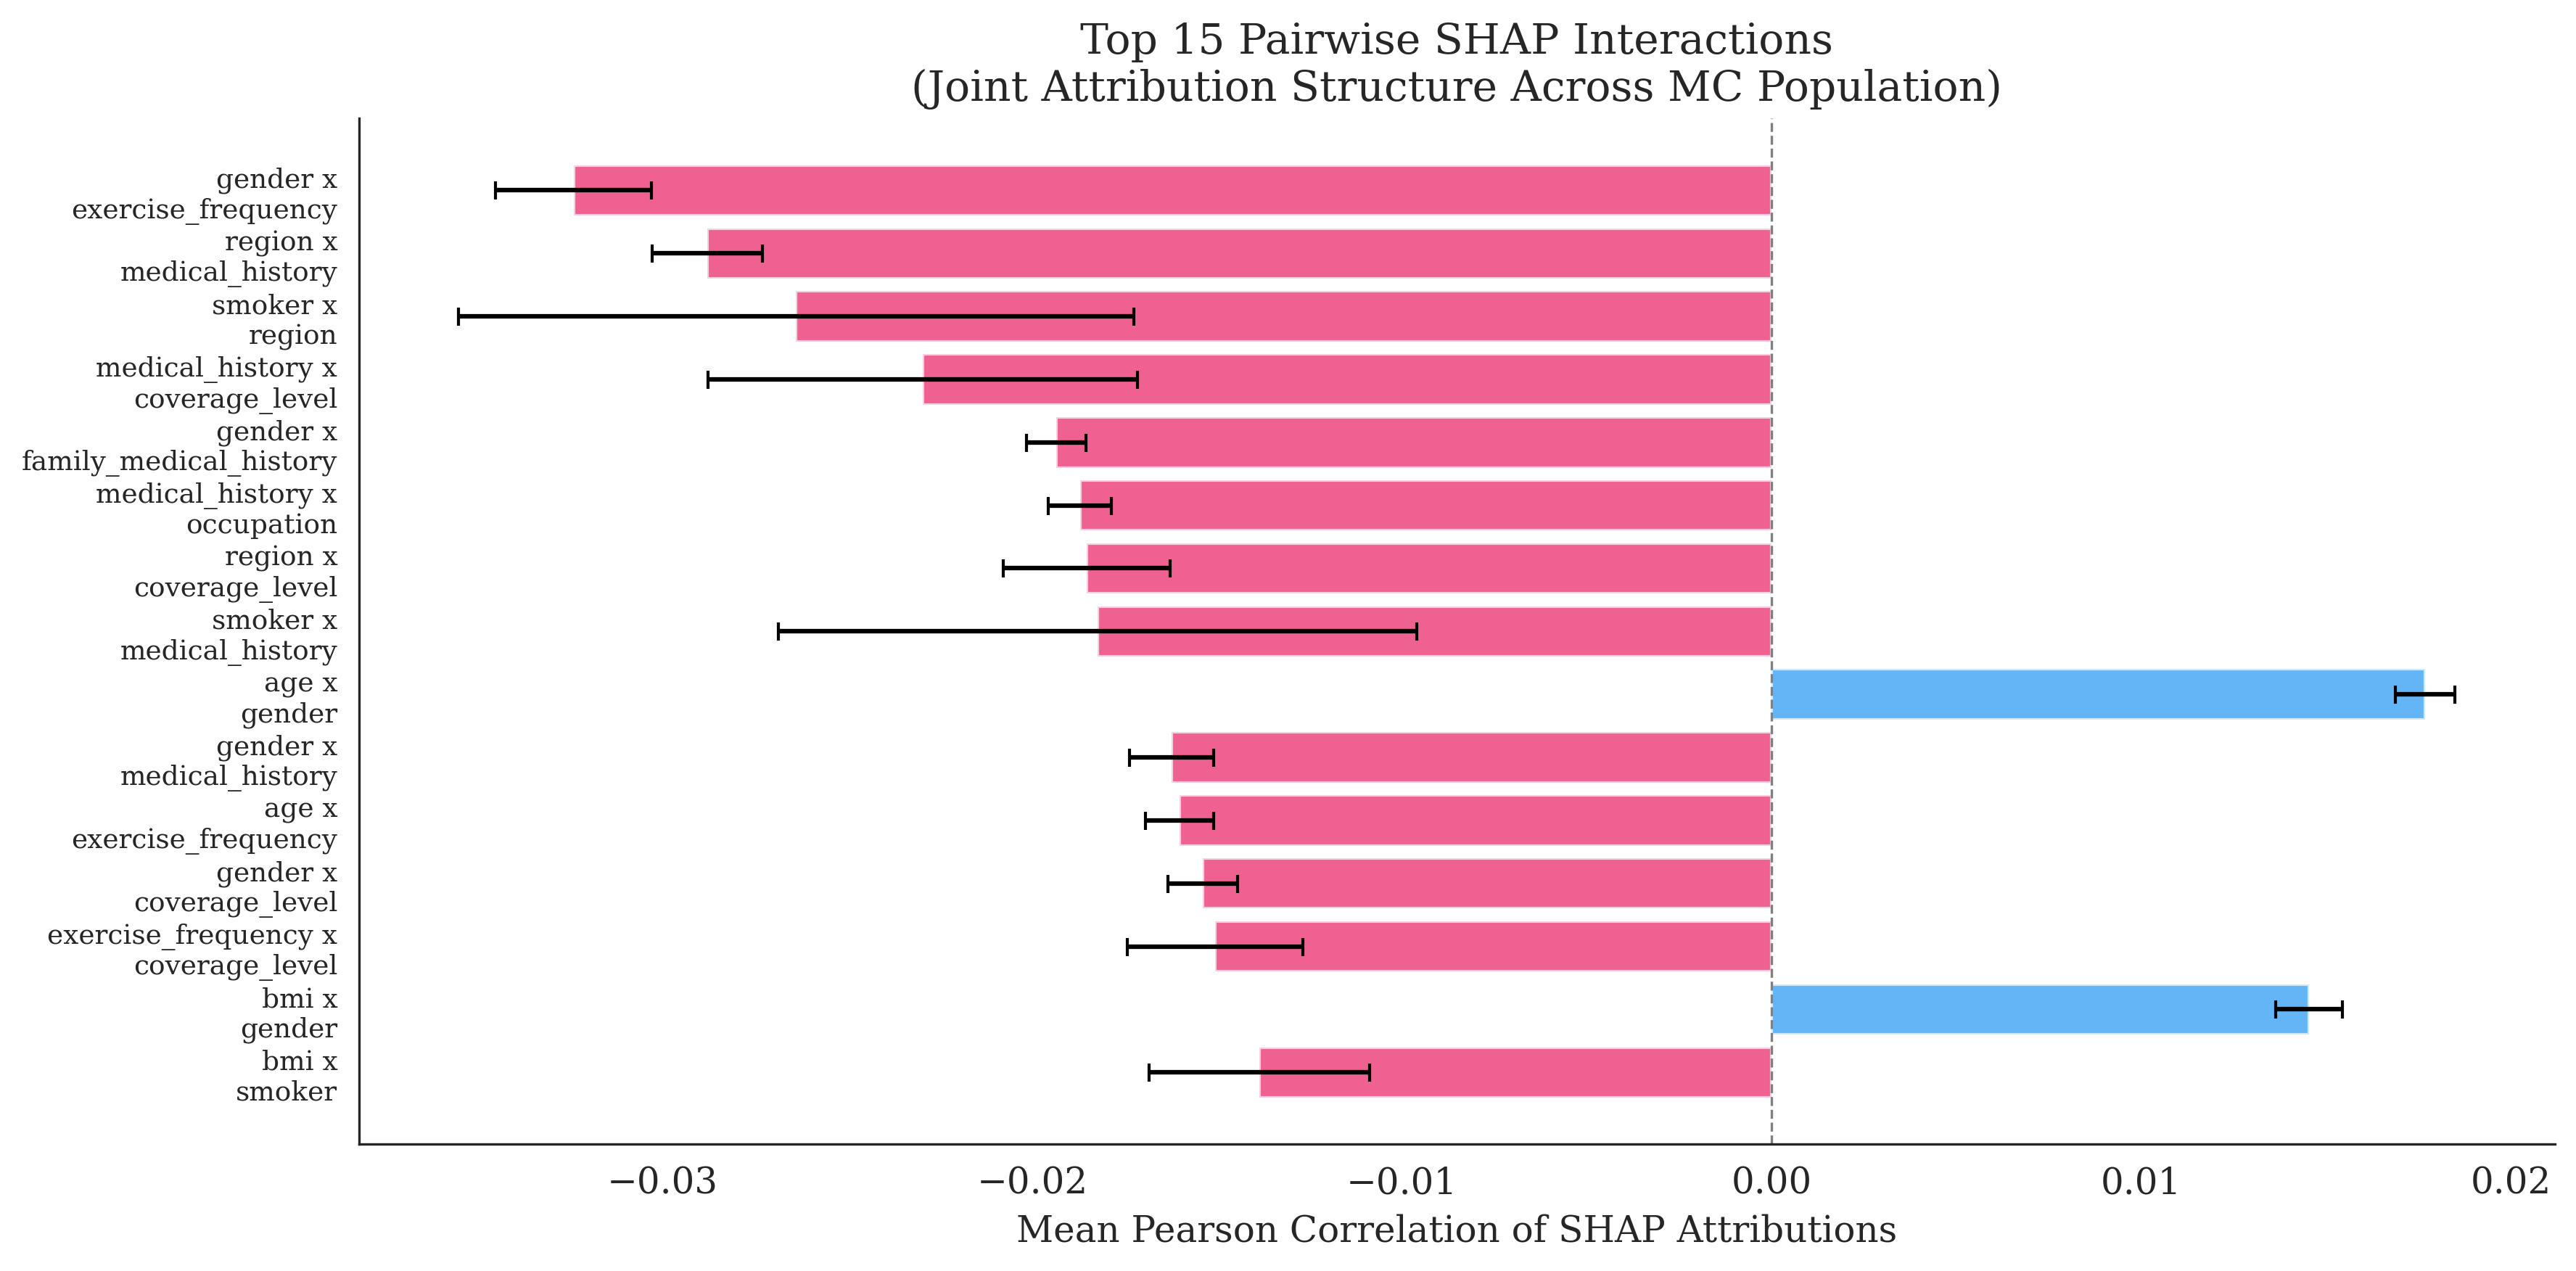
\includegraphics[width=0.80\textwidth]{Thesis/Chapter 4/Figures/fig_shap_interaction_pairs.png}
\caption{Top 15 pairwise SHAP interaction correlations.  All 55
pairwise correlations fall below $|r| = 0.033$, confirming that
the DNN has learned an essentially additive mapping.}
\label{fig:shap_interaction_pairs_annex}
\end{figure}
